%! Author = Philipp Emmenegger
%! Date = 10/06/2021

\section{Haskell Introduction}
\subsection{Standard Prelude}
\textbf{Select the first element of a list}
\begin{lstlisting}
head [1,2,3,4,5]
1
\end{lstlisting}
\textbf{Remove the first element of a list}
\begin{lstlisting}
tail [1,2,3,4,5]
[2,3,4,5]
\end{lstlisting}
\textbf{Select the nth element of a list}
\begin{lstlisting}
[1,2,3,4,5] !! 2
3
\end{lstlisting}
\textbf{Select the first n elements of a list}
\begin{lstlisting}
take 3 [1,2,3,4,5]
[1,2,3]
\end{lstlisting}
\textbf{Remove the first n elements from a list}
\begin{lstlisting}
drop 3 [1,2,3,4,5]
[4,5]
\end{lstlisting}
\textbf{Calculate the length of a list}
\begin{lstlisting}
length [1,2,3,4,5]
5
\end{lstlisting}
\textbf{Calculate the sum of a list of numbers}
\begin{lstlisting}
sum [1,2,3,4,5]
15
\end{lstlisting}
\textbf{Calculate the product of a list of numbers}
\begin{lstlisting}
product [1,2,3,4,5]
120
\end{lstlisting}
\textbf{Append two lists}
\begin{lstlisting}
[1,2,3] ++ [4,5]
[1,2,3,4,5]
\end{lstlisting}
\textbf{Reverse a list}
\begin{lstlisting}
reverse [1,2,3,4,5]
[5,4,3,2,1]
\end{lstlisting}

\subsection{Function Application Syntax}
\begin{lstlisting}
f a b + c * d
\end{lstlisting}
\begin{itemize}
    \item Function application is denoted using space
    \item Multiplication is denoted using $*$
    \item Function application has higher prio than other operators
\end{itemize}
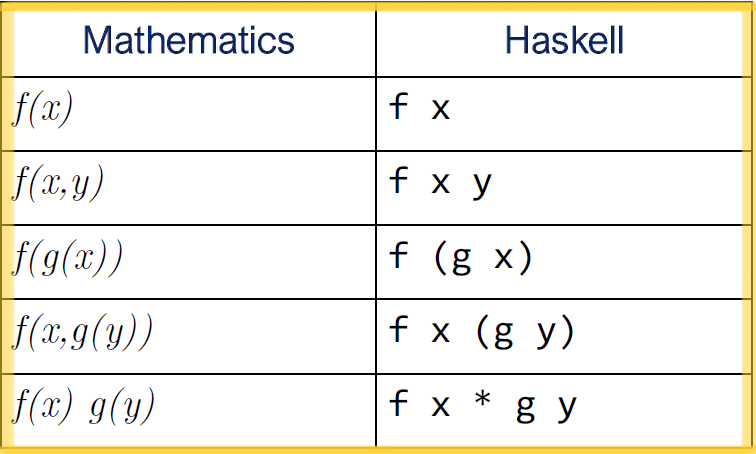
\includegraphics[width=0.6\linewidth]{../img/function_application_syntax.png}\\

\subsection{Useful GHCi Commands}
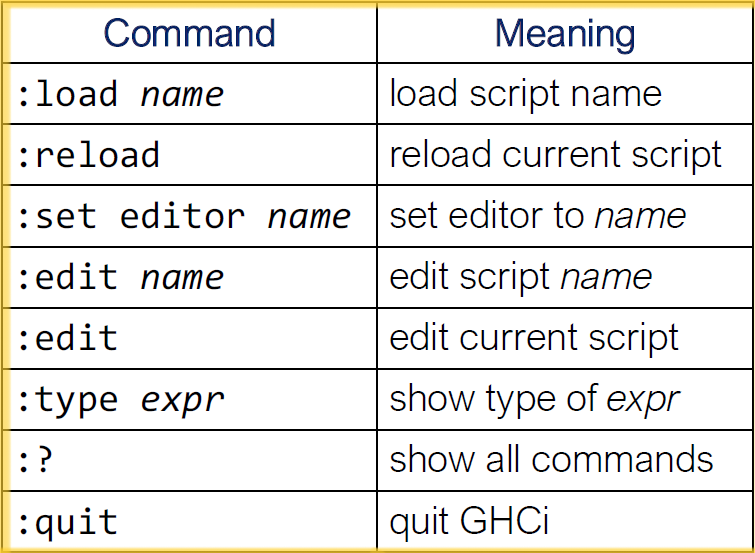
\includegraphics[width=0.6\linewidth]{../img/ghci_commands.png}\\

\subsection{Naming Requirements}
\begin{itemize}
    \item Function and argument names: begin with lowercase letter
    \item List arguments: $s$-suffix, by convention: $xs, ns, nss$
\end{itemize}

\subsection{The Layout Rule}
\begin{itemize}
    \item In a sequence of definitions, definitions must begin in the same column
    \item Avoids the need for braces and semicolons
\end{itemize}













